% Appendix generated from W&B-exported CIFAR-100 model-size curriculum runs.
\chapter{CIFAR-100 Model-Size Study for Coarse-to-Fine Curriculum Learning}
\label{app:cifar100-model-size-curriculum}

\section{Purpose}

This appendix summarizes the first CIFAR-100 model-size study for the
coarse-to-fine curriculum learning reproduction. The main question was whether
the curriculum remains useful as the model becomes larger or architecturally
stronger. A secondary goal was to check whether macro-F1, top-5 accuracy,
hierarchy-aware scores, and calibration tell the same story as top-1 accuracy.

The runs are best read as a screening study. They show where the curriculum is
promising and where it is not, but they do not by themselves settle questions of
statistical stability or optimization-landscape smoothness. The roughness and
sharpness diagnostics were not active in this batch, so the direct Hessian and
sharpness question is taken up in Appendix~\ref{app:roughness-followup-curriculum}.

\section{Experimental protocol}

The analysis uses 80 completed runs from the CIFAR-100 model-size sweep. The
runs were grouped by model, architecture family, and curriculum length before
aggregation.

The common training protocol was:

\begin{itemize}
    \item dataset: CIFAR-100,
    \item seed: 42,
    \item optimizer: Adam,
    \item learning rate: 0.001,
    \item scheduler: none,
    \item batch size: 128,
    \item training budget: 100 epochs,
    \item curriculum lengths: 5, 10, 20, 30, and 40 epochs,
    \item checkpoints disabled.
\end{itemize}

Each model configuration was run as a Figure-11-style sweep consisting of one
baseline and five curriculum runs. The omitted length 50 was intentionally not
used in this study, because earlier runs suggested that very long hard curricula
mostly delay fine-label specialization.

The analyzed model ladder consisted of:

\begin{itemize}
    \item width-scaled CNNs: \texttt{cnn\_w0.5}, \texttt{cnn\_w1},
          \texttt{cnn\_w2}, and \texttt{cnn\_w4},
    \item CIFAR-style ResNets with depths 8, 20, 32, and 56,
    \item ImageNet-style ResNet adapted to CIFAR: \texttt{resnet18}.
\end{itemize}

The \texttt{cnn\_w0.5} job appears to have been restarted several times on
Runpod before the auto-stop logic was corrected. These repeated runs have the
same seed and configuration, so they are not independent random seeds. For the
summary tables below, repeated runs with the same model and curriculum length
were averaged. All other model configurations have one run per curriculum
length.

Because this sweep is mostly single-seed, it should be interpreted as an
exploratory map of the effect rather than a final significance test. The
multi-seed follow-up in Appendix~\ref{app:roughness-followup-curriculum}
rechecks the most important CIFAR-100 cases.

\section{Primary results: curriculum benefit versus model size}

Table~\ref{tab:cifar100-model-size-best} reports, for each model, the best
curriculum length according to best test accuracy, its gain over the baseline,
and the corresponding AUC gain. Accuracy gains are shown in percentage points.

\begin{table}[h]
\centering
\small
\begin{tabular}{lrrrrrr}
\hline
Model & Params & Base & Best CL & CL acc. & Gain & AUC gain \\
\hline
\texttt{cnn\_w0.5} & 65,636 & 0.3478 & 20 & 0.3796 & +3.18 & -4.08 \\
\texttt{cifar\_resnet8} & 83,892 & 0.5268 & 20 & 0.5449 & +1.81 & -5.94 \\
\texttt{cnn\_w1} & 158,820 & 0.3849 & 10 & 0.4211 & +3.62 & -2.29 \\
\texttt{cifar\_resnet20} & 278,324 & 0.6028 & 10 & 0.6047 & +0.19 & -4.22 \\
\texttt{cnn\_w2} & 428,132 & 0.4256 & 5 & 0.4472 & +2.16 & -0.81 \\
\texttt{cifar\_resnet32} & 472,756 & 0.6172 & 10 & 0.6207 & +0.35 & -2.79 \\
\texttt{cifar\_resnet56} & 861,620 & 0.6314 & 20 & 0.6233 & -0.81 & -7.04 \\
\texttt{cnn\_w4} & 1,298,532 & 0.4463 & 5 & 0.4447 & -0.16 & -3.35 \\
\texttt{resnet18} & 11,220,132 & 0.6876 & 20 & 0.6937 & +0.61 & -6.44 \\
\hline
\end{tabular}
\caption{Best curriculum run per model on CIFAR-100. Gain and AUC gain are
reported in percentage points relative to the matching baseline.}
\label{tab:cifar100-model-size-best}
\end{table}

Here, ``best test accuracy'' means the best point reached along the test
trajectory. This is useful for understanding the learning dynamics, but it is
not a deployment-style model-selection rule. In a stricter protocol, the epoch
would be selected on validation data and the test set would be used only once at
the selected epoch. The AUC column is the normalized area under the per-epoch
test-accuracy curve; a negative AUC gain means that the curriculum spent much of
training below the baseline trajectory even if it later reached a better peak.

The strongest curriculum benefits occur in the smaller CNNs. The largest gain is
observed for \texttt{cnn\_w1} (+3.62 percentage points), followed by
\texttt{cnn\_w0.5} (+3.18 points) and \texttt{cnn\_w2} (+2.16 points). In
contrast, the largest CNN, \texttt{cnn\_w4}, no longer benefits. The CIFAR-style
ResNets also show a capacity-dependent pattern: \texttt{cifar\_resnet8} gains
+1.81 points, while \texttt{cifar\_resnet20} and \texttt{cifar\_resnet32} are
almost unchanged, and \texttt{cifar\_resnet56} is worse than baseline.

The ImageNet-style \texttt{resnet18} achieves the highest absolute accuracy and
shows a small positive best-accuracy gain (+0.61 points), but this gain is much
smaller than the gains seen in the smaller CNNs. Moreover, its AUC gain is
negative, which means that the curriculum run was not faster or better over the
whole training trajectory.

\begin{figure}[h]
    \centering
    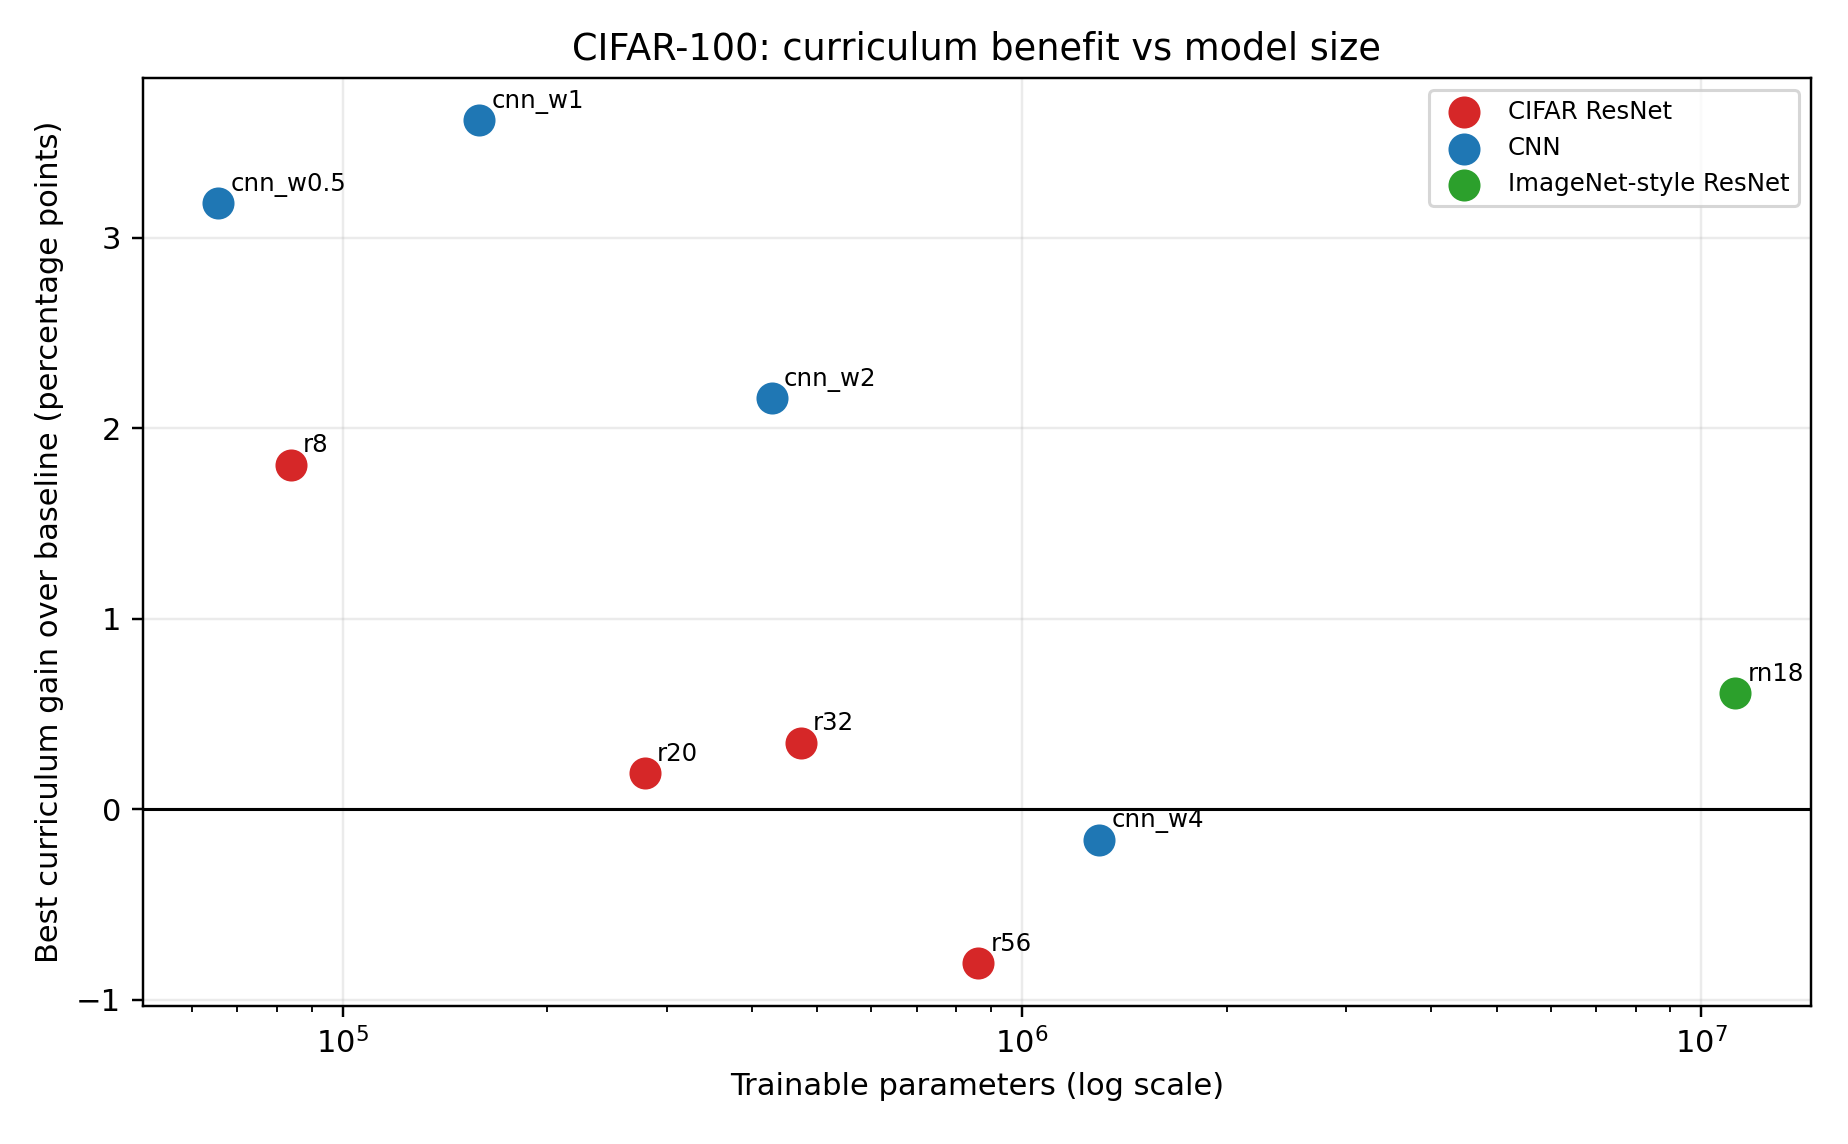
\includegraphics[width=0.90\textwidth]{figures/cifar100_model_size_gain_vs_params.png}
    \caption{Best curriculum gain over baseline as a function of trainable
    parameter count. The strongest gains occur for smaller CNNs, while larger
    CNNs and deeper CIFAR ResNets show little or negative benefit.}
    \label{fig:cifar100-model-size-gain-vs-params}
\end{figure}

\section{Curriculum length sensitivity}

Table~\ref{tab:cifar100-model-size-lengths} shows the best test accuracy for all
curriculum lengths. The baseline is represented as length 0.

\begin{table}[h]
\centering
\small
\begin{tabular}{lrrrrrr}
\hline
Model & Base & CL5 & CL10 & CL20 & CL30 & CL40 \\
\hline
\texttt{cnn\_w0.5} & 0.3478 & 0.3757 & 0.3783 & 0.3796 & 0.3729 & 0.3634 \\
\texttt{cifar\_resnet8} & 0.5268 & 0.5243 & 0.5321 & 0.5449 & 0.5228 & 0.5318 \\
\texttt{cnn\_w1} & 0.3849 & 0.4188 & 0.4211 & 0.4070 & 0.3820 & 0.3708 \\
\texttt{cifar\_resnet20} & 0.6028 & 0.5857 & 0.6047 & 0.5966 & 0.5869 & 0.5826 \\
\texttt{cnn\_w2} & 0.4256 & 0.4472 & 0.4250 & 0.4030 & 0.3824 & 0.3828 \\
\texttt{cifar\_resnet32} & 0.6172 & 0.6177 & 0.6207 & 0.6143 & 0.6143 & 0.6091 \\
\texttt{cifar\_resnet56} & 0.6314 & 0.6195 & 0.6224 & 0.6233 & 0.6218 & 0.6118 \\
\texttt{cnn\_w4} & 0.4463 & 0.4447 & 0.4319 & 0.4041 & 0.3950 & 0.3825 \\
\texttt{resnet18} & 0.6876 & 0.6884 & 0.6915 & 0.6937 & 0.6849 & 0.6871 \\
\hline
\end{tabular}
\caption{Best test accuracy by curriculum length on CIFAR-100.}
\label{tab:cifar100-model-size-lengths}
\end{table}

A clear qualitative pattern appears within the CNN family. As CNN width
increases, the best curriculum becomes shorter:

\begin{itemize}
    \item \texttt{cnn\_w0.5}: best at 20 curriculum epochs,
    \item \texttt{cnn\_w1}: best at 10 curriculum epochs,
    \item \texttt{cnn\_w2}: best at 5 curriculum epochs,
    \item \texttt{cnn\_w4}: no useful curriculum length.
\end{itemize}

This is consistent with the interpretation that smaller models need more help
from coarse supervision, while stronger CNNs need either only a short curriculum
or no hard curriculum at all.

\begin{figure}[h]
    \centering
    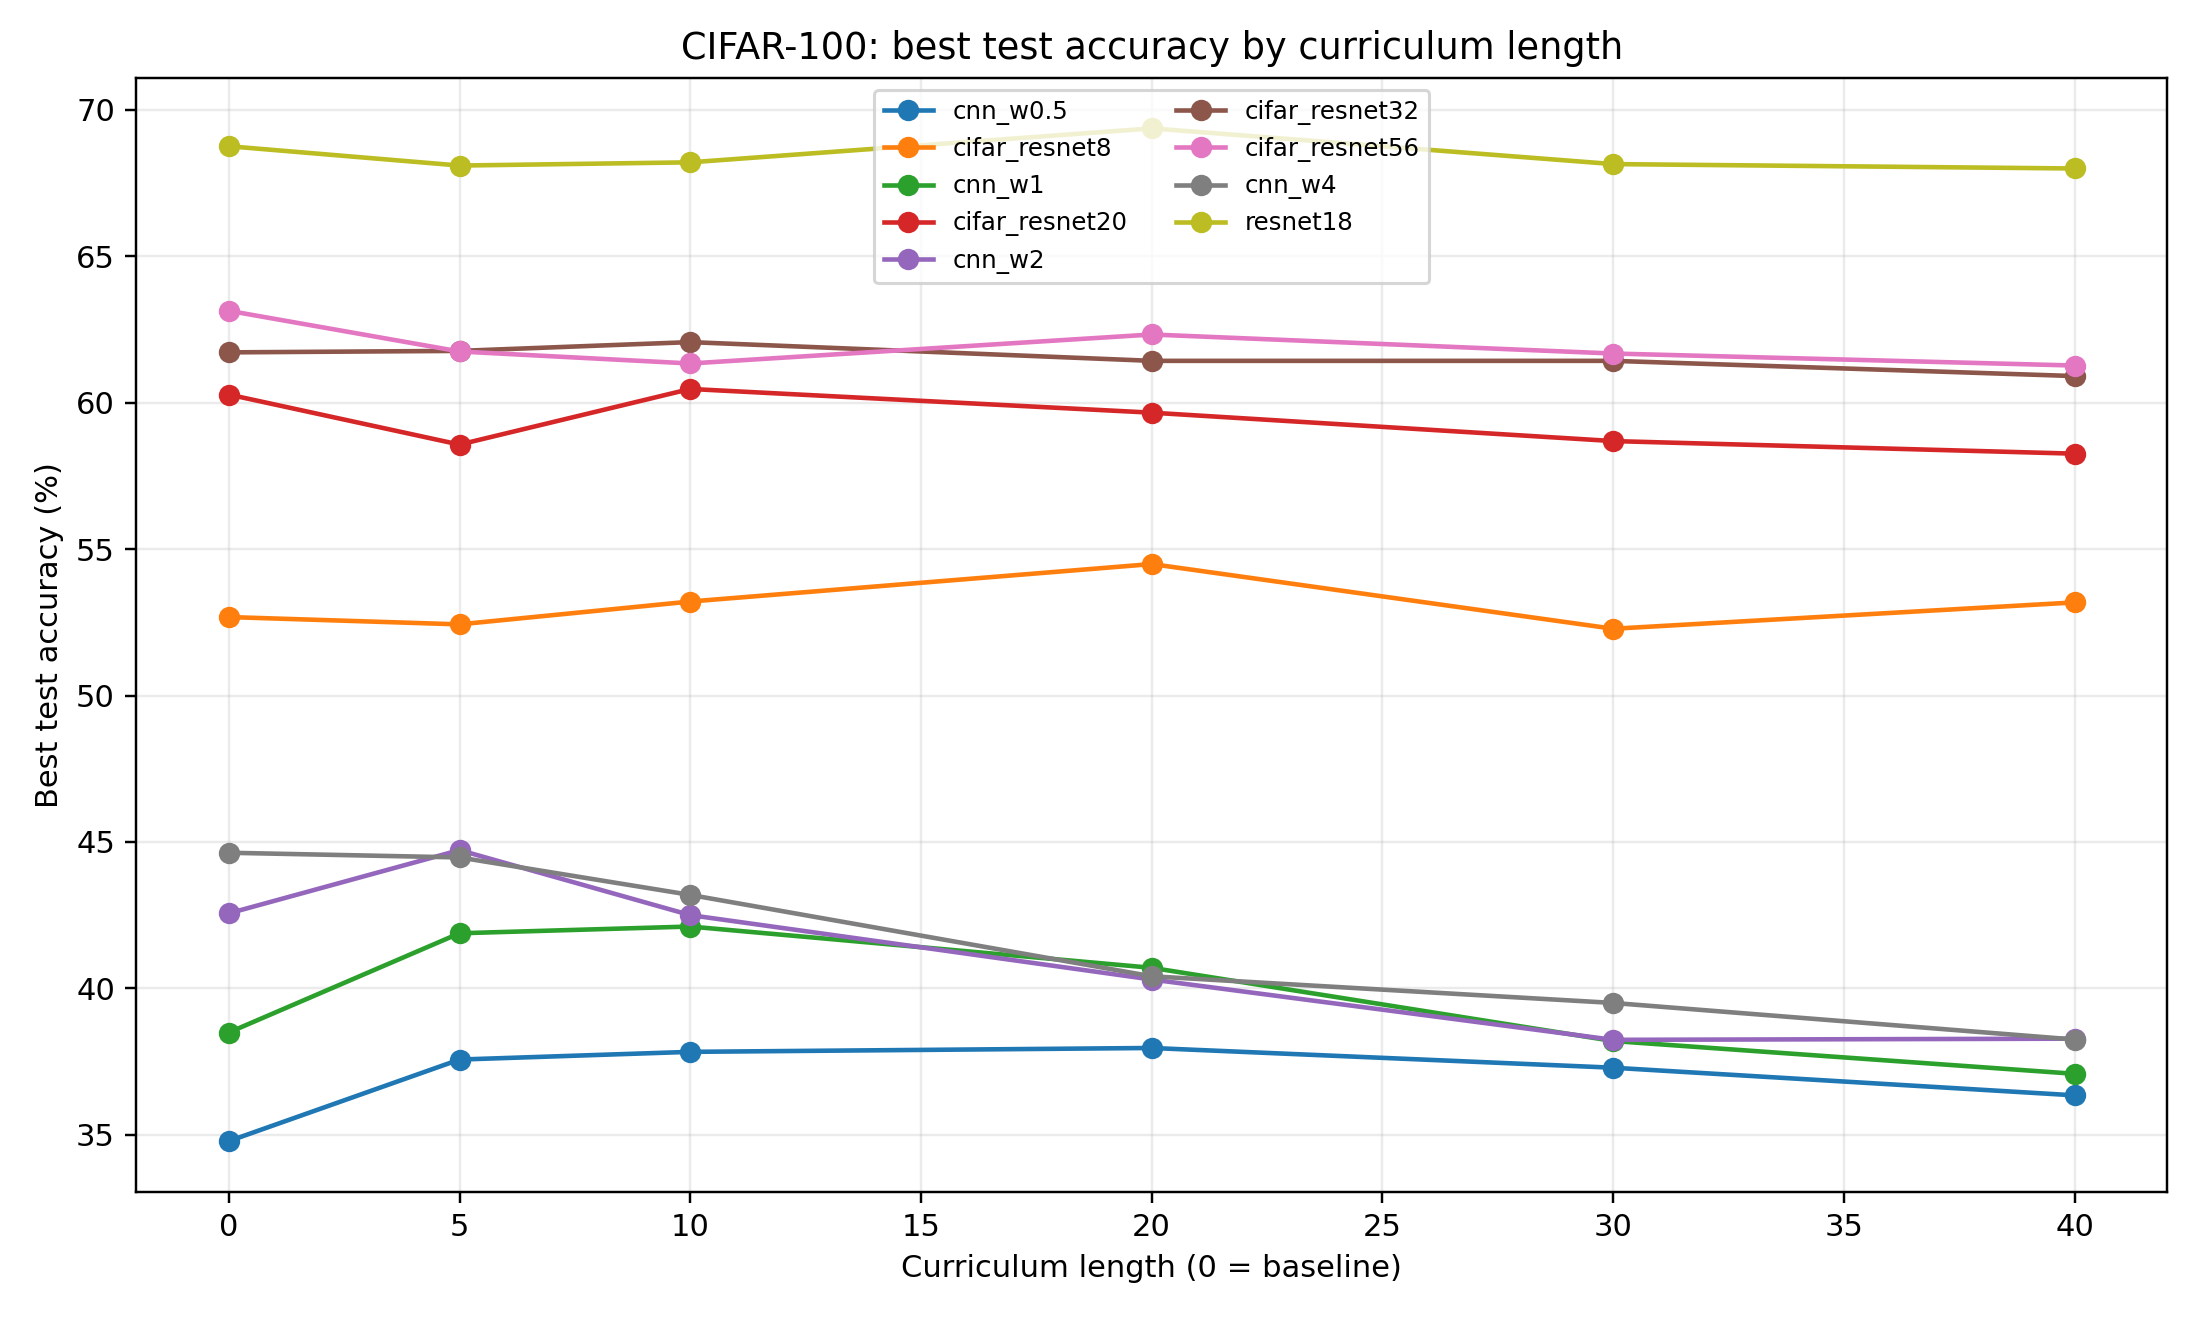
\includegraphics[width=0.95\textwidth]{figures/cifar100_model_size_curriculum_lengths.png}
    \caption{Best test accuracy by curriculum length. Length 0 denotes the
    baseline. Long curricula hurt most larger models, while small CNNs benefit
    from moderate curriculum lengths.}
    \label{fig:cifar100-model-size-curriculum-lengths}
\end{figure}

\section{Speed and AUC}

The curriculum runs generally do not improve the full test-accuracy trajectory.
Figure~\ref{fig:cifar100-model-size-auc-gain} shows the AUC gain for the best
curriculum run of each model. All values are negative.

\begin{figure}[h]
    \centering
    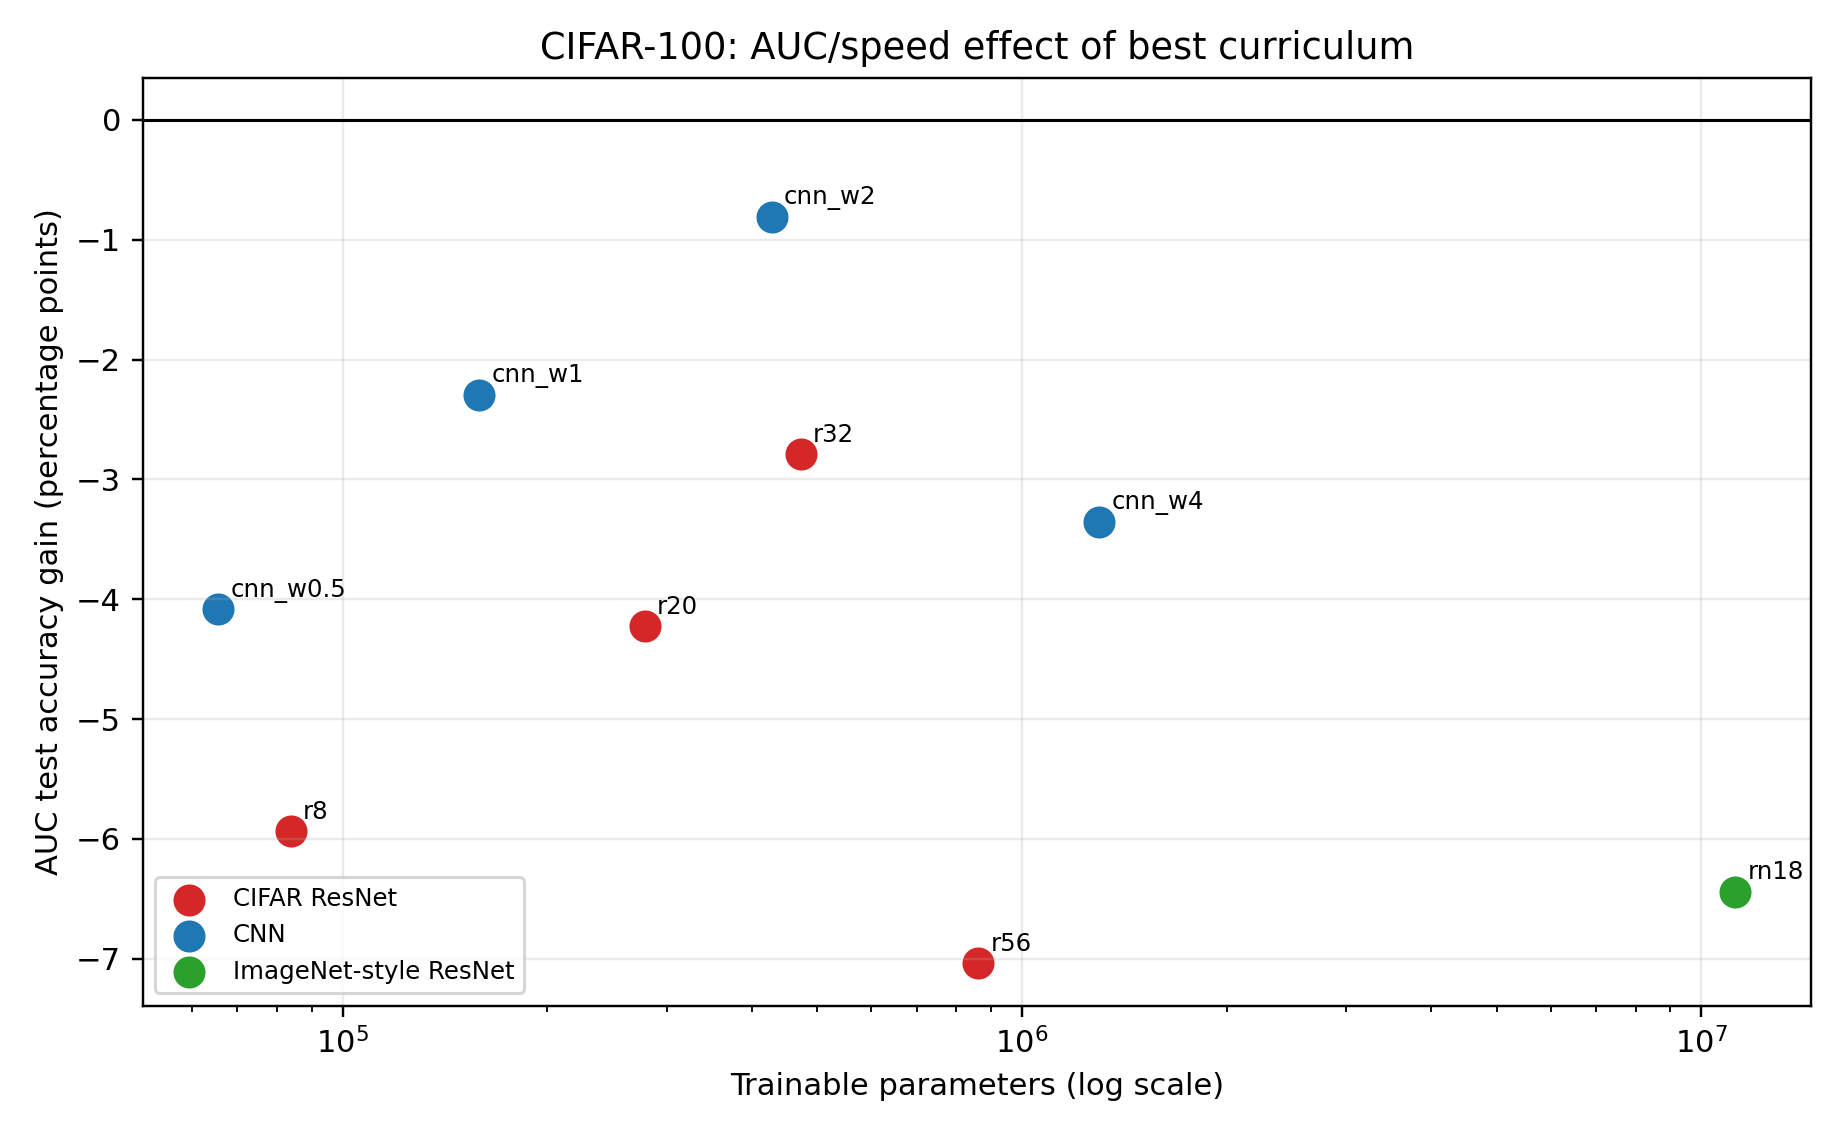
\includegraphics[width=0.90\textwidth]{figures/cifar100_model_size_auc_gain.png}
    \caption{AUC test-accuracy gain for the best curriculum run per model. The
    best curriculum can improve peak accuracy while still lowering AUC, because
    early coarse stages delay fine-label accuracy.}
    \label{fig:cifar100-model-size-auc-gain}
\end{figure}

This changes the interpretation of the curriculum effect. These runs do not show
that hard coarse-to-fine curriculum learning makes training uniformly faster.
Instead, the evidence suggests that curriculum can improve the best solution
encountered by smaller models, while sacrificing some early fine-label
performance.

\section{Metrics beyond accuracy}

The alternative metrics generally agree with the accuracy results. For the
models that benefit most in top-1 accuracy, curriculum also improves macro-F1,
top-5 accuracy, and hierarchy-aware scores. For models with weak or negative
accuracy gains, the alternative metrics are also weak or negative. The official
hierarchy-aware score gives partial credit when the prediction falls in the same
CIFAR-100 superclass as the target, so it measures whether mistakes remain close
in the human-defined class hierarchy.

\begin{table}[h]
\centering
\small
\begin{tabular}{lrrrrr}
\hline
Model & Acc. gain & F1 gain & Top-5 gain & Official hier. gain & ECE delta \\
\hline
\texttt{cnn\_w0.5} & +3.18 & +1.33 & +1.37 & +1.63 & +2.96 \\
\texttt{cifar\_resnet8} & +1.81 & +2.69 & +1.37 & +2.71 & -1.41 \\
\texttt{cnn\_w1} & +3.62 & +1.37 & +2.89 & +1.91 & +1.22 \\
\texttt{cifar\_resnet20} & +0.19 & -0.18 & +0.16 & -0.08 & -2.61 \\
\texttt{cnn\_w2} & +2.16 & +0.51 & +0.80 & +0.58 & +0.60 \\
\texttt{cifar\_resnet32} & +0.35 & +0.28 & +0.38 & +0.47 & -1.04 \\
\texttt{cifar\_resnet56} & -0.81 & -0.22 & -0.79 & -0.27 & -1.03 \\
\texttt{cnn\_w4} & -0.16 & -0.77 & -1.15 & -1.15 & +2.01 \\
\texttt{resnet18} & +0.61 & +0.37 & +0.44 & +0.44 & -0.48 \\
\hline
\end{tabular}
\caption{Alternative metric changes for the best curriculum run of each model.
All values except ECE are percentage-point gains relative to baseline. Negative
ECE delta indicates improved calibration.}
\label{tab:cifar100-model-size-alt-metrics}
\end{table}

The hierarchy-aware metrics are especially relevant because coarse-to-fine
curriculum learning is explicitly hierarchical. Figure~\ref{fig:cifar100-model-size-hier-gain}
compares exact top-1 gain against the official CIFAR-100 hierarchy-score gain.
Most models lie in the expected quadrants: when top-1 accuracy improves, the
hierarchical score also improves.

\begin{figure}[h]
    \centering
    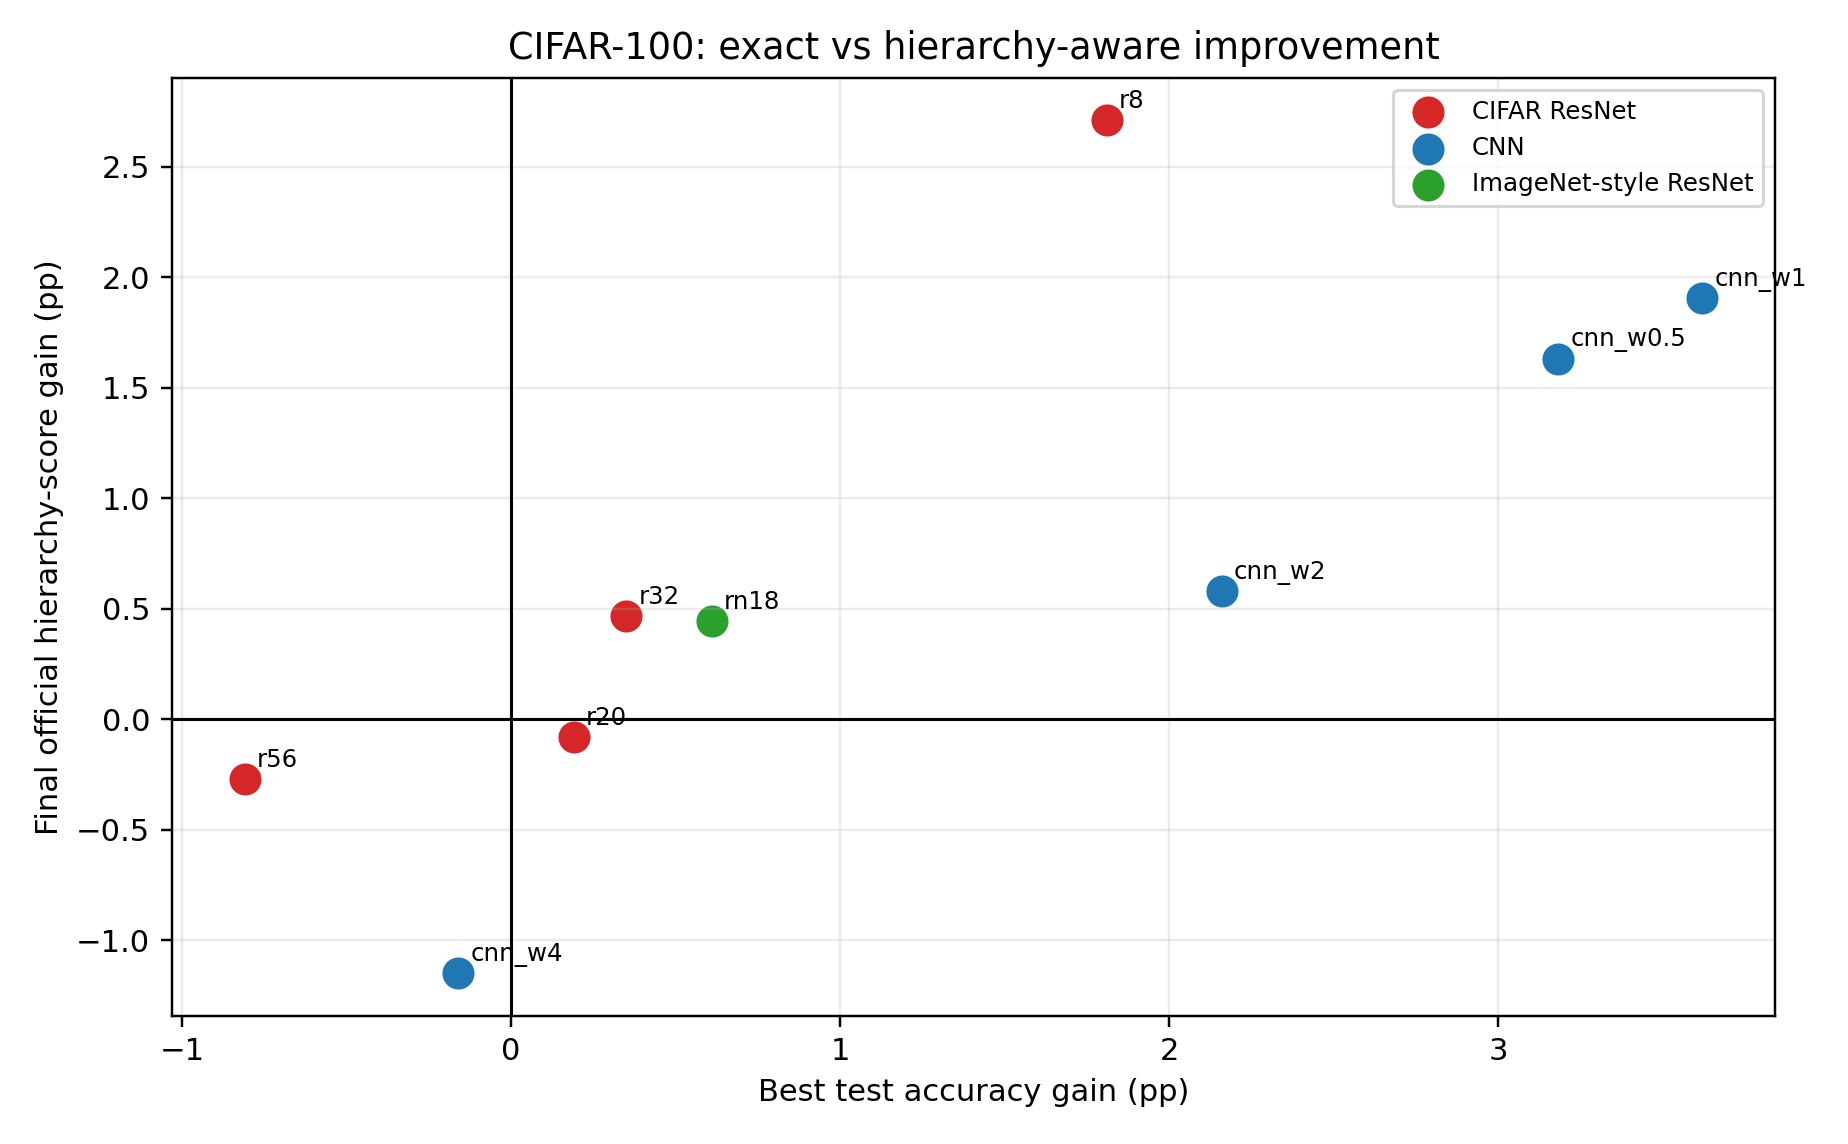
\includegraphics[width=0.90\textwidth]{figures/cifar100_model_size_hier_gain.png}
    \caption{Relationship between exact top-1 improvement and official
    hierarchy-score improvement. For the smaller models, curriculum improves both
    exact and hierarchy-aware behavior.}
    \label{fig:cifar100-model-size-hier-gain}
\end{figure}

Calibration behaves differently across architecture families. CNN curricula tend
to worsen ECE even when accuracy improves, suggesting more overconfident
predictions. CIFAR ResNets and ResNet-18 often show slightly improved ECE under
their best curriculum runs.

\section{Sharpness and landscape smoothness}

No direct conclusion about sharpness or optimization-landscape smoothing can be
drawn from this batch, because the roughness diagnostics were not active. This
is a limitation of the data collected here, not evidence for or against the
method itself. In particular, the accuracy gains in this appendix should not be
read as proof that the curriculum finds flatter minima. Appendix~\ref{app:roughness-followup-curriculum}
adds a focused roughness follow-up and shows that the picture is mixed.

\section{Interpretation}

The current evidence supports a capacity-conditioned view of hard
coarse-to-fine curriculum learning:

\begin{quote}
On CIFAR-100, hard coarse-to-fine curriculum learning is most useful for
low-capacity CNNs. As model width, residual depth, or architecture strength
increases, the benefit shrinks or disappears. The curriculum can improve peak
accuracy and hierarchy-aware behavior, but it usually does not improve the full
training trajectory as measured by AUC.
\end{quote}

This statement is stronger than a simple CNN-versus-ResNet comparison, because
there is now within-family evidence. In the CNN family, increasing width changes
the optimal curriculum from moderate length to short length and finally to no
benefit. In the CIFAR ResNet family, the smallest model benefits, while deeper
models show near-zero or negative gain.

The result should still be interpreted with care. The main sweep uses one random
seed, and architecture and capacity are not fully separable when comparing CNNs,
CIFAR ResNets, and ImageNet-style ResNet-18. The most defensible claim is
therefore that curriculum usefulness depends on both capacity and architecture,
with the strongest evidence for a within-family capacity effect in the CNN
models.

\section{Connection to the follow-up study}
\label{sec:cifar100-model-size-next-steps}

Appendix~\ref{app:roughness-followup-curriculum} follows this screening sweep in
three ways. First, it repeats the most important CIFAR-100 cases across three
seeds, so the single-seed pattern from this appendix can be checked for
stability. Second, it adds roughness and sharpness diagnostics for a smaller set
of representative models. Third, it tests whether the same curriculum idea
transfers to Fashion-MNIST, CIFAR-10, and Tiny ImageNet.

The main remaining gaps are now more targeted. The full model-size ladder was
not repeated across many seeds, and the reported peak test accuracy should be
complemented by test accuracy at the best validation epoch. The random-hierarchy
control is now covered in Appendix~\ref{app:hierarchy-ablation-curriculum},
which shows that matched random coarsening explains only part of the gain in the
main CIFAR-100 weak-CNN setting. The next open hierarchy question is broader:
how classifier-weight hierarchies compare with semantic or dataset-defined
hierarchies across multiple architectures.
